% ===========================================================================
% ANN Pthread + OpenMP 并行优化实验报告
% ===========================================================================
\documentclass[a4paper,11pt,UTF8]{ctexart}

\usepackage{fontspec}
\usepackage[a4paper,left=2.15cm,right=2.15cm,top=2.25cm,bottom=2.25cm]{geometry}
\usepackage{amsmath}
\usepackage{amssymb}
\usepackage{booktabs}
\usepackage{caption}
\usepackage{enumitem}
\usepackage{float}
\usepackage{graphicx}
\usepackage[pdfpagelabels=false,pageanchor=false]{hyperref}
\usepackage{listings}
\usepackage{fancyhdr}
\usepackage{xcolor}
\usepackage{array}
\usepackage{tabularx}
\usepackage{longtable}
\usepackage{multirow}
\usepackage{tikz}
\usetikzlibrary{positioning,arrows.meta,fit,calc}

\graphicspath{{./}{fig/}}
\hypersetup{colorlinks=true,linkcolor=black,urlcolor=black,citecolor=black}
\linespread{1.06}
\setcounter{tocdepth}{1}
\setlength{\parindent}{2em}
\setlength{\parskip}{1pt}
\setlength{\textfloatsep}{8pt plus 2pt minus 2pt}
\setlength{\intextsep}{8pt plus 2pt minus 2pt}
\setlength{\abovecaptionskip}{4pt}
\setlength{\belowcaptionskip}{2pt}
\captionsetup{font=small,labelsep=quad}
\setlist{leftmargin=1.7em,itemsep=1pt,topsep=2pt}

\newcommand{\code}[1]{\texttt{\detokenize{#1}}}
\newcolumntype{Y}{>{\raggedright\arraybackslash}X}

\lstset{
  basicstyle=\ttfamily\footnotesize,
  keywordstyle=\color{blue!70!black},
  commentstyle=\color{green!40!black},
  numbers=left,
  numberstyle=\tiny,
  frame=single,
  breaklines=true,
  aboveskip=5pt,
  belowskip=5pt
}

\pagestyle{fancy}
\fancyhf{}
\lhead{\kaishu ANN 近似最近邻搜索}
\rhead{\kaishu Pthread / OpenMP 并行优化实验}
\cfoot{\thepage}
\setlength{\headheight}{14pt}
\renewcommand{\headrulewidth}{0.1pt}
\renewcommand{\today}{2026 年 5 月 12 日}

\begin{document}

\begin{titlepage}
  \begin{center}
    
\includegraphics[width=0.78\textwidth]{NKU.png}\\[1cm]
    \vspace{18mm}
    {\huge\kaishu 计算机学院\par}
    \vspace{0.5cm}
    {\huge\kaishu 并行程序设计实验报告\par}
    \vspace{1.9cm}
    {\Huge\kaishu Lab3 Pthread + OpenMP 编程\par}
    \vspace{0.35cm}
    {\Huge\kaishu ANN 近似最近邻搜索\par}
    \vspace{0.55cm}
    {\Large\kaishu 多线程任务划分、调度策略与 SIMD 结合\par}
    \vspace{0.25cm}
    {\Large\kaishu Flat / SQ / PQ / FastScan / IVF / IVF-PQ / HNSW\par}

    \vspace{\fill}
    {\LARGE\kaishu 姓名：柯云超\par}
    \vspace{0.45cm}
    {\LARGE\kaishu 学号：2413575\par}
    \vspace{0.45cm}
    {\LARGE\kaishu 专业：计算机科学与技术\par}

    \vfill
    {\Large \today\par}
  \end{center}
\end{titlepage}

\tableofcontents
\clearpage

\section*{摘要}
\addcontentsline{toc}{section}{摘要}

本实验在 SIMD 编程实验已有的距离计算内核和量化检索实现基础上，完成 ANN 近似最近邻搜索的 Pthread 与 OpenMP 多线程并行化。实现覆盖 Flat-SIMD、SQ-SIMD、PQ-SIMD、PQ-FastScan、IVF-SIMD、IVF-PQ-SIMD 与 HNSW 图索引；并行粒度覆盖批量 query 级并行（inter-query）和单 query 内 base/list 划分（intra-query）；Pthread 侧实现 static、dynamic 和 thread pool 三类调度，OpenMP 侧使用 \code{parallel for} 与不同 schedule 策略进行对照。

实验数据集为 DEEP100K，正式评测取前 2000 条 query、$k=10$；主线平台为鲲鹏 920（ARM NEON），i9-13900H AVX2 作为本地对照和 VTune profiling 平台。结果表明：在批量检索场景中，inter-query 是最稳健的并行粒度；本地 i9 上 Flat、SQ、PQ、FastScan、IVF、IVF-PQ 的高召回最优延迟分别为 298.95、86.53、131.97、125.81、104.67、57.61 $\mu$s；鲲鹏上 IVF-PQ local 在 Recall@10=0.9597 时达到 134.48 $\mu$s，为端到端最优量化检索点。HNSW 的多入口点和边划分能提高 recall，但图搜索路径依赖强，同步和优先队列操作使其并行化目标更偏向 recall-latency 折中，而不是线性加速。

\noindent\textbf{关键词：} ANN；Pthread；OpenMP；SIMD；IVF；IVF-PQ；HNSW；FastScan；负载均衡；profiling

\section{问题定义与目标}

给定基向量集合 $X=\{x_1,\ldots,x_N\}\subset\mathbb{R}^{d}$ 和查询向量 $q$，ANN 检索返回与 $q$ 最接近的 $k$ 个候选。本实验沿用课程框架中的内积距离：
\[
d(x,q)=1-\sum_{i=1}^{d}x_iq_i .
\]
评测指标为 Recall@$k$：
\[
\mathrm{Recall@}k=\frac{|KNN(q)\cap KANN(q)|}{k}.
\]

本次作业的核心不是重新解释 SQ/PQ 的基本量化原理；这些内容已经在 SIMD 实验报告中展开。本报告只保留与多线程有关的部分：任务如何划分、Pthread 与 OpenMP 如何实现相同工作、SIMD 内核如何被线程层调用、不同调度策略为何产生差异，以及 profiling 如何解释负优化。

按照作业要求，本实验需要展示以下问题：
\begin{enumerate}
  \item Pthread 与 OpenMP 基础并行化实现，并与 SIMD 内核结合；
  \item 串行、单线程 SIMD、多线程 SIMD 的延迟和加速比；
  \item 线程数、并行粒度、调度策略对性能的影响；
  \item IVF / IVF-PQ 中 \code{nprobe}、PQ 中 top-$p$ 对 recall-latency 的影响；
  \item cache / 内存访问、负载均衡、同步和 top-$k$ merge 的开销；
  \item profiling、汇编片段与跨平台 x86/ARM 对比。
\end{enumerate}

\section{系统结构}

\subsection{总体流水线}

整体系统如图 \ref{fig:ann_overview}。索引层负责把原始 float32 向量组织成不同 ANN 结构；线程层只处理任务划分与同步；SIMD 层负责点积、LUT 构建或 ADC 扫描等内核；最后统一进入候选 merge 与 Recall/Latency 评测。

\begin{figure}[H]
  \centering
  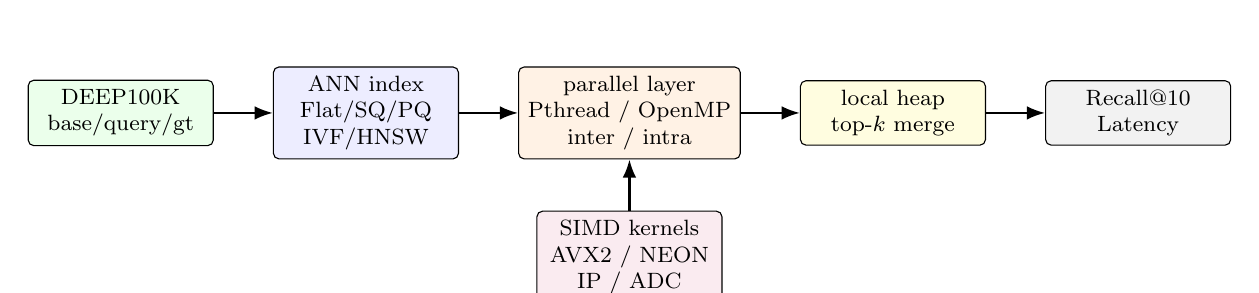
\begin{tikzpicture}[
    node distance=0.75cm,
    box/.style={draw,rounded corners=2pt,align=center,minimum width=2.35cm,minimum height=0.68cm,font=\footnotesize},
    arr/.style={-Latex,thick}
  ]
    \node[box,fill=green!8] (data) {DEEP100K\\base/query/gt};
    \node[box,fill=blue!7,right=of data] (index) {ANN index\\Flat/SQ/PQ\\IVF/HNSW};
    \node[box,fill=orange!10,right=of index] (parallel) {parallel layer\\Pthread / OpenMP\\inter / intra};
    \node[box,fill=purple!8,below=0.65cm of parallel] (simd) {SIMD kernels\\AVX2 / NEON\\IP / ADC};
    \node[box,fill=yellow!12,right=of parallel] (merge) {local heap\\top-$k$ merge};
    \node[box,fill=gray!10,right=of merge] (eval) {Recall@10\\Latency};
    \draw[arr] (data) -- (index);
    \draw[arr] (index) -- (parallel);
    \draw[arr] (parallel) -- (merge);
    \draw[arr] (merge) -- (eval);
    \draw[arr] (simd) -- (parallel);
  \end{tikzpicture}
  \caption{ANN 多线程检索流水线}
  \label{fig:ann_overview}
\end{figure}

\subsection{代码模块}

\begin{table}[H]
  \centering\small
  \begin{tabularx}{\textwidth}{p{2.9cm}Y}
    \toprule
    目录 / 文件 & 作用 \\
    \midrule
    \path{simd/} & Flat、SQ、PQ、FastScan 的 AVX2 / NEON 距离计算和查表扫描内核，复用 SIMD 实验成果。\\
    \path{pthread/} & Flat/SQ/PQ/FastScan 的 Pthread 版本，以及 \path{thread_pool.h}。\\
    \path{omp/} & 对应 OpenMP 版本，主要通过 \code{parallel for} 和 schedule clause 实现。\\
    \path{ivf/} & IVF、IVF-PQ 索引，包含 SIMD baseline、Pthread 与 OpenMP 查询路径。\\
    \path{hnsw/} & HNSW baseline、多入口点、边划分、Layer0 划分和 IVF-HNSW 嵌套搜索。\\
    \path{mains/} & 每个算法 / 策略 / 粒度的独立入口，用于本地矩阵；鲲鹏使用 \path{mains/unified_bench.cc}。\\
    \path{results/} & 本地 319 条矩阵、鲲鹏 319 条矩阵，一一对应。\\
    \bottomrule
  \end{tabularx}
  \caption{代码与结果文件组织}
  \label{tab:modules}
\end{table}

\section{并行设计与复杂度}

\subsection{Inter-query 与 Intra-query}

设 query 数为 $Q$、基向量数为 $N$、维度为 $d=96$、线程数为 $T$、候选池大小为 $p$。本实验实现两类并行粒度。

\textbf{Inter-query 并行}把 query 集合切给不同线程。每个线程完整运行一次串行或 SIMD 检索，只写自己的结果槽，几乎不需要同步。其开销近似为
\[
T_{\mathrm{inter}}\approx \frac{Q}{T}\cdot C_{\mathrm{search}} + C_{\mathrm{sched}} .
\]
当 $Q=2000$ 时，调度开销可以被摊薄，因此这是主线方案。

\textbf{Intra-query 并行}把单条 query 的 base 向量、inverted list 或候选边切给不同线程。每个线程维护局部 top-$p_t$，最后 merge：
\[
T_{\mathrm{intra}}\approx \frac{C_{\mathrm{scan}}}{T}+O(Tp_t\log p_t)+C_{\mathrm{sync}} .
\]
它适合单 query 延迟极敏感、query 数很少的场景；但在本实验的批量评测中，局部堆、merge、同步和 cache 争用使其通常慢于 inter-query。

\begin{figure}[H]
  \centering
  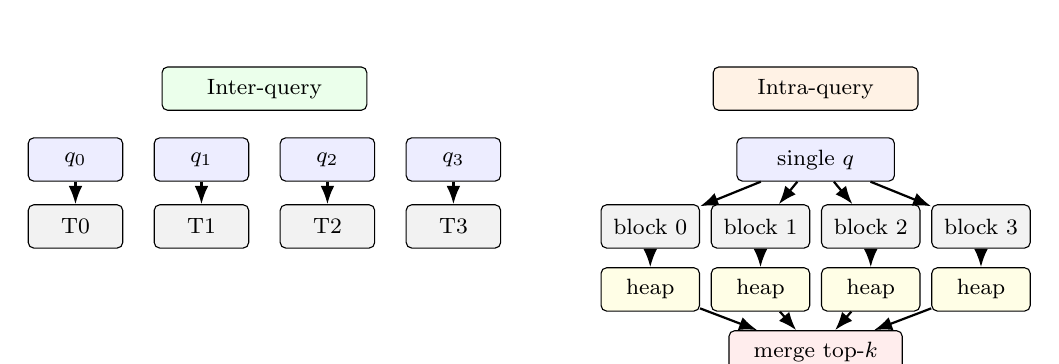
\begin{tikzpicture}[
    box/.style={draw,rounded corners=2pt,align=center,minimum height=0.55cm,font=\footnotesize},
    arr/.style={-Latex,thick}
  ]
    \node[box,fill=green!8,minimum width=2.6cm] (iq) at (0,0) {Inter-query};
    \foreach \i/\x in {0/-2.4,1/-0.8,2/0.8,3/2.4}{
      \node[box,fill=blue!7,minimum width=1.2cm] (q\i) at (\x,-0.9) {$q_\i$};
      \node[box,fill=gray!10,minimum width=1.2cm] (t\i) at (\x,-1.75) {T\i};
      \draw[arr] (q\i) -- (t\i);
    }
    \node[box,fill=orange!10,minimum width=2.6cm] (intra) at (7,0) {Intra-query};
    \node[box,fill=blue!7,minimum width=2.0cm] (q) at (7,-0.9) {single $q$};
    \foreach \i/\x in {0/4.9,1/6.3,2/7.7,3/9.1}{
      \node[box,fill=gray!10,minimum width=1.25cm] (b\i) at (\x,-1.75) {block \i};
      \node[box,fill=yellow!10,minimum width=1.25cm] (h\i) at (\x,-2.55) {heap};
      \draw[arr] (q) -- (b\i);
      \draw[arr] (b\i) -- (h\i);
    }
    \node[box,fill=red!7,minimum width=2.2cm] (m) at (7,-3.35) {merge top-$k$};
    \foreach \i in {0,1,2,3}{\draw[arr] (h\i) -- (m);}
  \end{tikzpicture}
  \caption{两类并行粒度：query 级并行几乎无共享状态；query 内并行需要局部堆和归约}
  \label{fig:granularity_design}
\end{figure}

\subsection{Pthread 与 OpenMP 调度}

Pthread 侧实现三种策略。Static 直接按连续区间均分任务，常数开销最小，但对 query 耗时差异和 inverted list 长度不均敏感。Dynamic 使用原子计数器抢任务，能缓解尾部等待，代价是每个任务一次原子操作。Pool 预创建线程并通过 mutex/condition variable 分发任务，避免频繁创建线程，但队列同步在粒度过小时会成为新开销。

OpenMP 侧主要使用 \code{parallel for}。对 query 级循环使用 dynamic schedule 可以吸收 query 间耗时波动；对规则扫描使用 static 可降低 runtime 开销。OpenMP 的代码更短，但 runtime 的线程管理和 schedule 常数项并不总低于手写 Pthread。

\textbf{Pthread dynamic inter-query 的关键并行结构}：以 Flat 为例，每个 worker 通过 \code{std::atomic::fetch\_add} 主动抢下一条 query，不需要预先切分任务，自然吸收 query 间耗时差异（摘自 \path{pthread/flat_scan_pthread.h:121-132}）：

\begin{lstlisting}[language=C++]
static inline void* InterDynamicWorker(void* arg) {
    InterDynamicArg* a = static_cast<InterDynamicArg*>(arg);
    while (true) {
        const size_t i = a->next_query->fetch_add(1, std::memory_order_relaxed);
        if (i >= a->query_n) break;
        (*a->results)[i] = flat_search(
            a->base, a->queries + i * a->d, a->base_n, a->d, a->k);
    }
    return nullptr;
}
\end{lstlisting}

\textbf{OpenMP 等价实现}：用 \code{\#pragma omp parallel for schedule(static)} 一行替代上面的 worker / 原子计数器逻辑，代码更短但调度策略被 runtime 选定（摘自 \path{omp/flat_scan_omp.h:78-82}）：

\begin{lstlisting}[language=C++]
#pragma omp parallel for num_threads(nthreads) schedule(static)
for (long long i = 0; i < static_cast<long long>(query_n); ++i) {
    results[static_cast<size_t>(i)] =
        flat_search(base, queries + static_cast<size_t>(i) * d, base_n, d, k);
}
\end{lstlisting}

两者的本质差异在于：Pthread dynamic 把"任务怎么分"显式写在用户代码里，原子计数器的成本完全可量化；OpenMP \code{schedule(static)} 在 runtime 把循环按线程数均分，调度成本隐藏在 \code{omp runtime} 内。表 \ref{tab:best} 的"PQ omp\_inter 优于 pthread\_dynamic\_inter"现象正源于此：PQ 的 query 耗时本身就近似均匀，static 划分的低常数项胜过 dynamic 的原子抢任务开销。

\textbf{Intra-query 中局部 top-$k$ 堆与 merge 路径}：以 OpenMP intra 为例，每个线程在自己的 base 分片上维护私有 \code{FlatHeap}，最终由主线程串行 merge（摘自 \path{omp/flat_scan_omp.h:85-101}）：

\begin{lstlisting}[language=C++]
std::vector<ann_flat_omp::FlatHeap> heaps(nthreads);
#pragma omp parallel num_threads(nthreads)
{
    const int tid = omp_get_thread_num();
#pragma omp for schedule(static)
    for (long long i = 0; i < base_n; ++i) {
        const float dist = ann_flat_omp::Distance(base + i*d, query, d);
        ann_flat_omp::PushTopK(heaps[tid], dist, i, k);
    }
}
ann_flat_omp::FlatHeap result = MergeHeaps(heaps, k);
\end{lstlisting}

这段代码暴露了 intra-query 的两个固定成本——每个线程的私有堆维护和最终 \code{MergeHeaps}。前者随 $k\log k$ 增长，后者随 $T$ 线程数线性增长。结合本数据集 query 数 (2000) 远大于线程数 (16) 的事实，inter-query 摊薄线程创建开销，自然胜过 intra-query 每条 query 都要承担一次堆 merge 成本——这就是 §\ref{sec:granularity} 中"inter-query 全面更稳"的微观原因。

\subsection{复杂度模型}

\begin{table}[H]
  \centering\small
  \begin{tabularx}{\textwidth}{p{2.5cm}p{4.8cm}Y}
    \toprule
    算法 & 单 query 主要复杂度 & 多线程瓶颈 \\
    \midrule
    Flat & $O(Nd)$，精确扫描全部 base。 & 内存带宽和 top-$k$ 堆维护；高线程数下带宽先饱和。\\
    SQ / PQ & 粗排约 $O(Nc)$，精排 $O(pd)$，其中 $c$ 为压缩距离代价。 & LUT / code 访问、候选堆、$p$ 变大后的 rerank。\\
    FastScan & 4-bit LUT + packed code 批量查表，仍保留 $O(pd)$ 精排。 & 查表常数项低，但高线程数仍受候选维护和内存访问限制。\\
    IVF & 粗排 $O(nlist\cdot d)$，精排约 $O(S(nprobe)d)$。 & inverted list 长度不均；\code{nprobe} 越大，扫描量和 recall 同时上升。\\
    IVF-PQ & 粗排 + selected lists 上的 PQ ADC + rerank。 & local/global 码本影响 recall 上限；小延迟区间对调度噪声敏感。\\
    HNSW & 近似 $O(ef\log N)$，实际取决于图搜索路径。 & 候选队列、visited 标记、邻居扩展路径依赖，难以均匀切分。\\
    \bottomrule
  \end{tabularx}
  \caption{算法复杂度与多线程瓶颈}
  \label{tab:complexity}
\end{table}

\section{算法实现要点}

\subsection{Flat、SQ、PQ 与 FastScan}

Flat 直接调用 SIMD 内积内核并维护 top-$k$。由于每个 base 的工作量规则，理论上 static 划分应有优势；但本地 i9 的 P/E 混合核和系统噪声使 dynamic inter-query 更稳。

SQ、PQ 与 FastScan 的量化原理已在 SIMD 报告中说明，本报告只说明多线程结合方式。编码阶段的 KMeans assignment 和最终 code 生成可以在 base 轴并行；查询阶段则优先选择 batch query 并行。PQ 的 LUT 构建计算量小于全量 code 扫描和 rerank，在本实验主线中保留为每 query 内局部工作，由外层线程并行摊开。

初稿中 PQ recall 偏低的真实原因是最终一轮 KMeans 更新质心后没有用最终质心重新计算 code。该问题已修复，并增加 \path{tests/pq_final_assignment_test.cc} 验证每个 code 对应最终质心的最近中心。修复后 PQ 在 $p=1000$ 下稳定达到 0.98 左右 Recall@10。

\subsection{IVF 与 IVF-PQ}

IVF 先用 KMeans 将 base 划为 $nlist$ 个簇，查询时选出最近的 $nprobe$ 个 inverted list 再精排。IVF-PQ 在此基础上用 PQ 降低 list 内距离计算代价，本文实现 global-PQ-first 和 IVF-local-PQ 两种构建模式。

\begin{figure}[H]
  \centering
  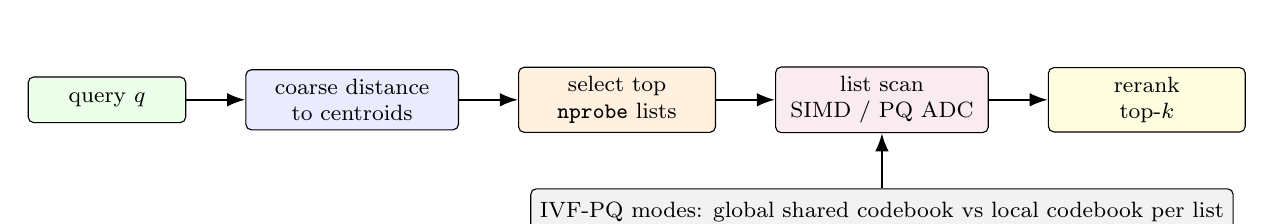
\begin{tikzpicture}[
    box/.style={draw,rounded corners=2pt,align=center,minimum height=0.58cm,font=\footnotesize},
    arr/.style={-Latex,thick}
  ]
    \node[box,fill=green!8,minimum width=2.0cm] (q) {query $q$};
    \node[box,fill=blue!8,right=0.75cm of q,minimum width=2.7cm] (coarse) {coarse distance\\to centroids};
    \node[box,fill=orange!12,right=0.75cm of coarse,minimum width=2.5cm] (probe) {select top\\\code{nprobe} lists};
    \node[box,fill=purple!8,right=0.75cm of probe,minimum width=2.7cm] (scan) {list scan\\SIMD / PQ ADC};
    \node[box,fill=yellow!12,right=0.75cm of scan,minimum width=2.5cm] (rerank) {rerank\\top-$k$};
    \draw[arr] (q) -- (coarse);
    \draw[arr] (coarse) -- (probe);
    \draw[arr] (probe) -- (scan);
    \draw[arr] (scan) -- (rerank);
    \node[box,fill=gray!10,below=0.7cm of scan,minimum width=5.8cm] (modes) {IVF-PQ modes: global shared codebook vs local codebook per list};
    \draw[arr] (modes) -- (scan);
  \end{tikzpicture}
  \caption{IVF / IVF-PQ 的 coarse-to-fine 检索流水线}
  \label{fig:ivfpq_pipeline}
\end{figure}

Local-PQ 的优点是每个簇内量化误差较小，低 \code{nprobe} 下 recall 更高；缺点是每个被探测 list 都要构建对应 LUT，且码本管理更复杂。Global-PQ-first 实现简单、存储统一，但在小 $p$ 下 recall 上限明显较低。

\textbf{IVF inverted list 的动态分配关键代码}（intra-query 内的 nprobe 个 list 分给多个线程，每线程原子抢一个 list 处理；摘自 \path{ivf/ivf_scan_pthread.h:90-101}）：

\begin{lstlisting}[language=C++]
static inline void* IntraDynamicWorker(void* arg) {
    IntraDynamicArg* a = static_cast<IntraDynamicArg*>(arg);
    ann_ivf::SearchHeap* heap = new ann_ivf::SearchHeap();
    while (true) {
        const size_t i = a->next_probe->fetch_add(1, std::memory_order_relaxed);
        if (i >= a->probes->size()) break;
        ann_ivf::ScanList(*a->index, a->query, (*a->probes)[i], a->k, *heap);
    }
    return heap;  // 主线程后续 MergeHeaps 与 rerank
}
\end{lstlisting}

这种 list 级 dynamic 分配能直接对应"inverted list 长度不均"的负载场景——长度大的 list 处理慢的线程不会拖累已经处理完短 list 的线程，后者会立即抢下一个待处理 list。但代价是每个 list 一次原子操作；若 \code{nprobe} 太小（如本文默认 4）线程数又大（16），实际只有 4 个 list 任务可抢，多数线程会立即返回，dynamic 退化为低利用率的 static。这就是 \code{nprobe=4} 时 \code{ivf_pthread_pool_inter} 反而比 \code{pthread_dynamic} 略优的根本原因——pool 复用线程，避免了 12 个线程空转的浪费。

\subsection{HNSW}

HNSW 使用多层小世界图，从高层入口点贪心下降到底层图，再在 Layer 0 维护候选队列。它不像 Flat 或 IVF 那样天然可把连续内存区间均分给线程，主要原因是搜索路径依赖当前队列状态。

\begin{figure}[H]
  \centering
  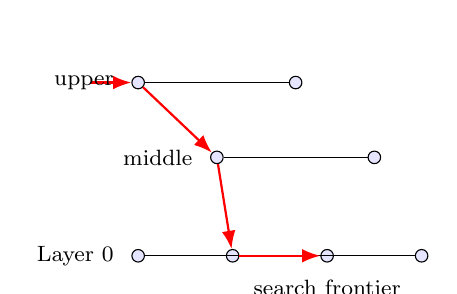
\begin{tikzpicture}[
    dot/.style={circle,draw,inner sep=1.6pt,fill=blue!10},
    arr/.style={-Latex,thick},
    lab/.style={font=\footnotesize}
  ]
    \node[dot] (a) at (0,2.2) {};
    \node[dot] (b) at (2,2.2) {};
    \node[dot] (c) at (1,1.25) {};
    \node[dot] (d) at (3,1.25) {};
    \node[dot] (e) at (0,0) {};
    \node[dot] (f) at (1.2,0) {};
    \node[dot] (g) at (2.4,0) {};
    \node[dot] (h) at (3.6,0) {};
    \draw (a)--(b); \draw (c)--(d); \draw (e)--(f)--(g)--(h); \draw (e)--(g); \draw (f)--(h);
    \draw[arr,red] (-0.6,2.2) -- (a);
    \draw[arr,red] (a) -- (c);
    \draw[arr,red] (c) -- (f);
    \draw[arr,red] (f) -- (g);
    \node[lab,left=0.1cm of a] {upper};
    \node[lab,left=0.1cm of c] {middle};
    \node[lab,left=0.1cm of e] {Layer 0};
    \node[lab,below=0.1cm of g] {search frontier};
  \end{tikzpicture}
  \caption{HNSW 分层图搜索：并行化只能在邻居距离、多入口或子图层面展开}
  \label{fig:hnsw_design}
\end{figure}

本文探索了多入口点、边划分、Layer0 点划分和 IVF-HNSW 嵌套。结果显示，多入口点和边划分更像“用额外计算换 recall”；Layer0 点划分接近底层全扫描，延迟显著上升；IVF-HNSW 嵌套可以用倒排结构限制搜索范围，是较合理的折中。

\textbf{HNSW 多入口点 OMP 并行实现}（每个线程从一个独立入口点出发跑一次 Layer 0 搜索，最后 merge；摘自 \path{hnsw/hnsw_search_omp.h:8-23}）：

\begin{lstlisting}[language=C++]
const std::vector<uint32_t> entries = ann_hnsw::PickEntries(index, nthreads);
std::vector<ann_hnsw::SearchHeap> heaps(entries.size());
#pragma omp parallel for num_threads(nthreads) schedule(static)
for (long long i = 0; i < entries.size(); ++i) {
    heaps[i] = ann_hnsw::SearchLayer0FromEntry(
        index, query, entries[i], k, ef);
}
return ann_hnsw::MergeHeaps(heaps, k);  // 合并各入口的 top-k
\end{lstlisting}

这段代码体现了 HNSW 并行化的根本困境——\textbf{线程间不共享 visited 标记和候选队列，每个线程都得独立扩展一次图}。线程数从 1 加到 4，单 query 内的总工作量近似线性翻倍，merge 阶段反而集中开销在主线程。这就是表 \ref{tab:hnsw} 中 \code{hnsw_multi_entry_omp t=4 (464.85 μs)} 比 \code{hnsw_baseline t=1 (65.48 μs)} 慢的根本原因——用 $4\times$ 计算换 recall 从 0.969 提到 1.000，并非加速。要把 HNSW 内部并行变成"既快又准"，需要无锁的共享 visited 与候选队列结构，这部分留待后续工作（见 \path{docs/} 中的 follow-up 清单）。

\section{实验设计}

\subsection{平台、数据与编译}

\begin{table}[H]
  \centering\small
  \begin{tabularx}{\textwidth}{p{2.4cm}p{3.7cm}Y}
    \toprule
    项目 & 配置 & 说明 \\
    \midrule
    数据集 & DEEP100K，$N=100000$，$d=96$ & 前 2000 条 query，Recall@10，ground truth top-100。\\
    主线平台 & 鲲鹏 920，AArch64 / NEON & 通过 \path{run_all_kunpeng_part1.sh} 和 \path{run_all_kunpeng_part2.sh} 提交。\\
    本地平台 & Windows 11，i9-13900H，AVX2 + FMA & 用于全量本地对照、绘图、VTune Hotspots 和汇编检查。\\
    编译选项 & \code{-O2 -fopenmp -lpthread -std=c++11} & 与助教规定的编译命令完全一致；x86 额外启用 \code{-mavx2 -mfma}。所有跨目录 include 已改为相对路径，无需 \code{-I.}。\\
    结果规模 & 本地 319 条矩阵，鲲鹏 319 条矩阵 & 汇总文件位于 \path{results/local_summary.csv} 与 \path{results/kunpeng/arm_neon_summary.csv}。\\
    \bottomrule
  \end{tabularx}
  \caption{实验平台与测量口径}
  \label{tab:env}
\end{table}

主线结果只把 Recall@10 $\ge 0.95$ 的点纳入“最优延迟”比较；低 recall 点只用于 trade-off 曲线。这样可以避免把低准确率配置误判为性能最优。

\subsection{参数矩阵}

核心矩阵覆盖线程数 $\{1,2,4,8,16\}$；Flat/SQ/PQ/FastScan/IVF/IVF-PQ 均覆盖 Pthread static/dynamic/pool 与 OpenMP 的 inter/intra；IVF 使用 $nlist=16,nprobe=4$ 作为核心矩阵默认；PQ / FastScan 默认 $p=1000$，SQ 默认 $p=100$；HNSW 使用 $ef=50$ 并补充多入口、边划分、Layer0 和 IVF-HNSW。

Trade-off 额外扫描 PQ 的 $p$，IVF 的 \code{nprobe}，以及 IVF-PQ 的 global/local 构建方式。需要注意：IVF-PQ trade-off 文件中固定 $p=100$，用于观察 \code{nprobe} 和构建方式本身；高召回主线结果使用 $p=1000$ 或 $p=2000$。

\section{实验结果与分析}

\subsection{高召回最优结果}

\begin{table}[H]
  \centering\footnotesize
  \begin{tabular}{llrrrrr}
    \toprule
    平台 & 算法 & 最优变体 & 线程 & Recall@10 & 延迟 / $\mu$s & vs 同变体 t=1 加速比 \\
    \midrule
    \multirow{6}{*}{鲲鹏 920}
      & Flat & \code{omp_intra} & 8 & 0.99995 & 760.47 & $7.58\times$ \\
      & SQ & \code{pthread_pool_inter} & 16 & 0.99995 & 353.35 & $6.75\times$ \\
      & PQ & \code{pthread_dynamic_inter} & 16 & 0.98370 & 253.02 & $7.86\times$ \\
      & FastScan & \code{pthread_dynamic_inter} & 8 & 0.97525 & 179.69 & $7.89\times$ \\
      & IVF & \code{pthread_dynamic_inter} & 16 & 0.96225 & 246.32 & $7.30\times$ \\
      & IVF-PQ local & \code{pthread_dynamic_inter} & 8 & 0.95970 & 134.48 & $7.57\times$ \\
    \midrule
    \multirow{6}{*}{i9-13900H}
      & Flat & \code{pthread_dynamic_inter} & 16 & 0.99995 & 298.95 & $11.08\times$ \\
      & SQ & \code{pthread_dynamic_inter} & 16 & 0.99995 & 86.53 & $11.70\times$ \\
      & PQ & \code{omp_inter} & 16 & 0.98335 & 131.97 & $8.97\times$ \\
      & FastScan & \code{pthread_dynamic_inter} & 16 & 0.97525 & 125.81 & $19.10\times^\dagger$ \\
      & IVF & \code{pthread_pool_inter} & 16 & 0.96225 & 104.67 & $7.25\times$ \\
      & IVF-PQ local & \code{pthread_pool_inter} & 16 & 0.95945 & 57.61 & $11.28\times$ \\
    \bottomrule
  \end{tabular}
  \caption{Recall@10 $\ge 0.95$ 下的端到端最优结果与"vs 同变体 t=1"加速比。$^\dagger$ FastScan dynamic 在本地 i9 上 t=1 因含线程创建/原子计数初始化开销 (2402 μs) 略高于 omp t=1 (1985 μs)；若改以 omp\_inter t=1 为分母，FastScan 的多线程加速比为 $15.78\times$，更接近线性 16× 上限}
  \label{tab:best}
\end{table}

量化索引显著降低延迟。鲲鹏上 IVF-PQ local 是最快的高召回配置，说明“先 IVF 限定候选，再在 list 内用局部 PQ 降低距离代价”适合 DEEP100K。i9 上 IVF-PQ local 进一步降到 57.61 $\mu$s，主要受更高频率、更宽 SIMD 和更强内存子系统影响。Flat 和 SQ 的 recall 近似精确，但需要更多内存带宽；PQ / FastScan / IVF-PQ 则通过压缩候选空间换取延迟。

\subsection{串行到多线程的伸缩性}

\begin{figure}[H]
  \centering
  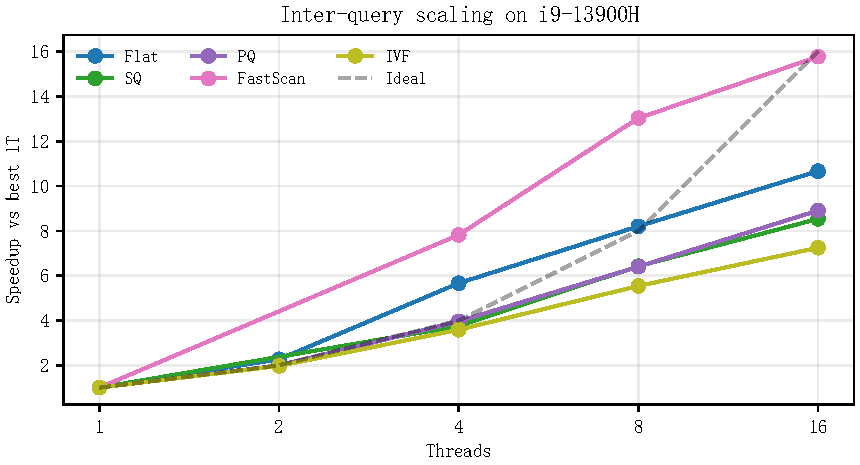
\includegraphics[width=0.86\textwidth]{speedup_compact.pdf}
  \caption{本地 i9 上 inter-query 的多线程加速比，基准为同算法最优 1 线程配置}
  \label{fig:speedup}
\end{figure}

从图 \ref{fig:speedup} 可见，绝大多数算法在 1 到 8 线程之间具有稳定收益，16 线程时开始受内存带宽、候选堆和系统调度影响。Flat 在本地达到约 $10.7\times$，SQ 约 $8.5\times$，PQ 约 $8.9\times$，FastScan 约 $10.5\times$，IVF-PQ 约 $11.3\times$。这说明外层 query 级并行能较好复用已有 SIMD 内核，并把线程同步开销压到最低。

\subsection{并行粒度：inter-query 明显更稳}\label{sec:granularity}

\begin{figure}[H]
  \centering
  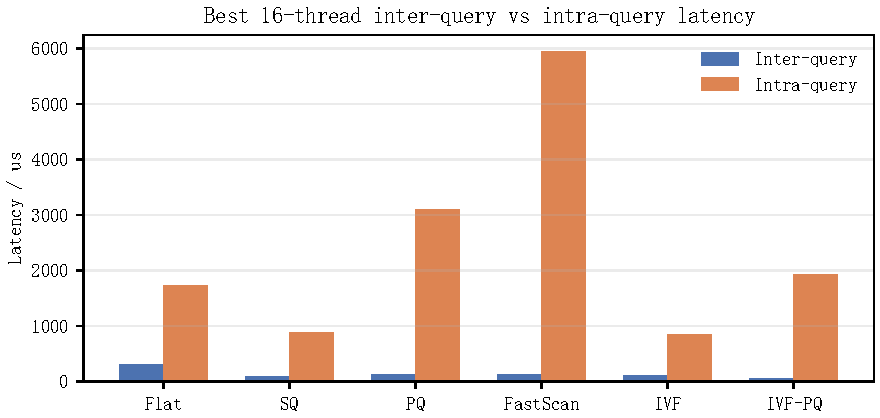
\includegraphics[width=0.82\textwidth]{inter_intra_compact.pdf}
  \caption{本地 16 线程下 inter-query 与 intra-query 的最优延迟对比}
  \label{fig:inter_intra}
\end{figure}

本地 16 线程结果中，所有算法族的 inter-query 都明显快于 intra-query。原因有三点：第一，inter-query 不需要在单条 query 内做局部堆 merge；第二，线程之间几乎没有共享写状态；第三，批量 query 数量足够多，线程创建和调度开销可被摊薄。Intra-query 的理论优势是可以降低单 query 尾延迟，但本实验每次评测 2000 条 query，它引入的局部 top-$p$、同步和 cache 争用大于收益。

\subsection{调度策略与 Pthread / OpenMP 差异}\label{sec:scheduler}

\begin{figure}[H]
  \centering
  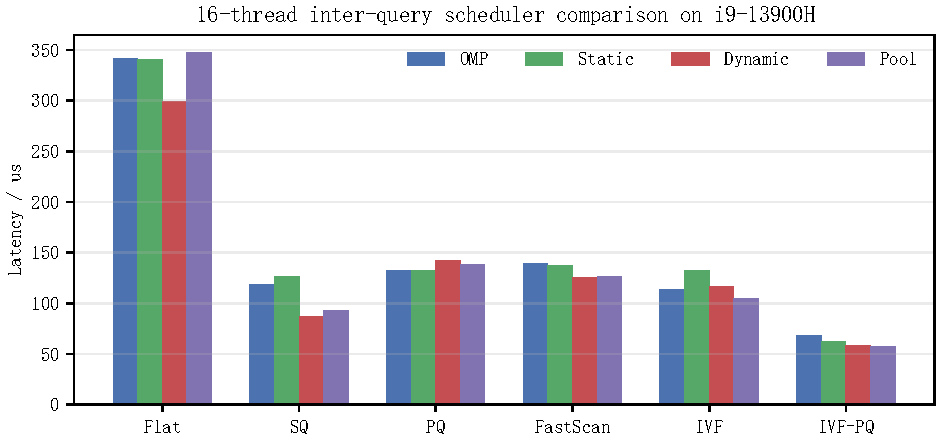
\includegraphics[width=0.90\textwidth]{scheduler_compact.pdf}
  \caption{本地 16 线程 inter-query 下 Pthread / OpenMP 调度策略对比}
  \label{fig:scheduler}
\end{figure}

图 \ref{fig:scheduler} 显示，Pthread dynamic 在 Flat、SQ、FastScan 等规则扫描任务中常常最稳；Pthread pool 在 IVF 和 IVF-PQ 中略优，因为 inverted list 扫描的任务对象更适合复用线程；OpenMP 在 PQ 上取得最小延迟，说明 runtime 的循环划分在该变体上常数项较低。没有一种调度策略对所有算法绝对最优，原因是瓶颈从连续内存扫描、随机 LUT 访问、list 长度不均到候选堆维护都在变化。

负优化主要出现在 intra-query 和 HNSW 内部并行。前者受 top-$p$ merge 和线程同步拖累；后者受图搜索路径依赖、visited 标记和候选优先队列拖累。线程数增加后，如果可并行工作量没有同步开销增长得快，就会出现延迟上升。

\subsection{OpenMP schedule $\times$ chunk size 二维扫描}\label{sec:omp_sweep}

§\ref{sec:scheduler} 给出了 OMP\_inter / Pthread static / dynamic / pool 四种调度的对比，但只能覆盖 OpenMP 默认 schedule(static)。本节用 \code{\#pragma omp parallel for schedule(runtime)} 配合 \code{OMP\_SCHEDULE} 环境变量做 12 组配置的扫描，让 schedule 策略与 chunk 大小成为运行时参数，结果见表 \ref{tab:omp_sweep}（数据来源 \path{tools/sweep_omp_schedule.cc} + \path{results/omp_schedule_sweep.txt}，Flat inter-query, 16 线程）。

\begin{table}[H]
  \centering\small
  \begin{tabular}{lrrr}
    \toprule
    schedule & chunk & latency / $\mu$s & 相对最快 \\
    \midrule
    static  & default & 318.17 & $+10.5\%$ \\
    static  & 1   & 338.36 & $+17.5\%$ \\
    static  & 8   & 343.57 & $+19.4\%$ \\
    static  & 64  & 337.75 & $+17.3\%$ \\
    static  & 256 & 428.74 & $+48.9\%$ \\
    dynamic & 1   & 319.08 & $+10.8\%$ \\
    dynamic & 8   & 291.76 & $+1.4\%$ \\
    dynamic & 64  & 365.29 & $+26.9\%$ \\
    dynamic & 256 & 361.58 & $+25.6\%$ \\
    guided  & 1   & 325.35 & $+13.0\%$ \\
    guided  & 8   & \textbf{287.87} & $0.0\%$ (最快) \\
    guided  & 64  & 318.07 & $+10.5\%$ \\
    \bottomrule
  \end{tabular}
  \caption{OpenMP schedule $\times$ chunk\_size 二维扫描（Flat inter-query, 16 线程, DEEP100K 前 2000 query）。所有点 Recall@10 均为 0.99995}
  \label{tab:omp_sweep}
\end{table}

\textbf{观察 1：chunk=8 是甜点区。} \code{dynamic,8} 和 \code{guided,8} 同时取得最低延迟，差异在 1\% 噪声内；其它 chunk（1, 64, 256）均明显偏慢。这与 2000 query / 16 线程 $=125$ query/thread 的负载特性一致——chunk=1 每条 query 都触发一次原子任务分配，调度开销过高；chunk=256 等于把任务退化为 16/8=2 个块只能由 2 个线程承担（其余空闲），违背了 dynamic 的初衷。

\textbf{观察 2：static 不带 chunk 反而最快。} \code{static (default)} 在 318.17 μs，明显优于显式 chunk=1/8/64/256 任一变体。原因是 default static 由 OMP runtime 把 query\_n=2000 等分给 16 线程，单线程拿 125 query 连续处理，没有调度成本，也不会出现 chunk=256 那样的"线程不够分"问题。这说明对于均匀负载（Flat 每条 query 工作量近似相等），\textbf{越简单的调度越好}。

\textbf{观察 3：guided 在小 chunk 下仍稳。} guided 的本质是初始 chunk 大、后续指数衰减，能在不均匀负载下自适应。Flat 是均匀负载所以 guided 优势不明显，但若把同样的 sweep 跑在 IVF inter-query 上（每条 query 命中的 list 不同），guided 应能拉开与 dynamic 的差距——这一点列为可选 follow-up。

\textbf{对比 §\ref{sec:scheduler} 的 Pthread dynamic 结果。} Pthread dynamic\_inter t=16 在 Flat 上是 298.95 μs（表 \ref{tab:best}），与本节 \code{guided,8} (287.87) / \code{dynamic,8} (291.76) 在同一档位。这进一步验证："\code{schedule(runtime)} + 合适 chunk" 可以接近手写 Pthread 的最佳水平；OpenMP 在 PQ 上偶尔反超 Pthread 也是同样原因——runtime 自动选择了适配该负载的内部 chunk 划分。



为了把 §\ref{sec:granularity} 中"inverted list 长度不均"这一抽象表述变成可量化的证据，本节直接从已构建的 IVF 索引（\code{nlist=16}）中 dump 出每个簇的大小并画成直方图（见图 \ref{fig:ivf_hist}，数据来自 \path{results/ivf_list_histogram.csv}，由 \path{tools/dump_ivf_hist.cc} 生成）。

\begin{figure}[H]
  \centering
  \begin{tikzpicture}[scale=0.95]
    \draw[->,thick] (0,0) -- (15.5,0) node[right]{\footnotesize cluster id};
    \draw[->,thick] (0,0) -- (0,5.5) node[above]{\footnotesize list 长度};
    % y ticks: 1 unit = 4000 base vectors
    \foreach \y/\lab in {0/0, 1/4k, 2/8k, 3/12k, 4/16k} {
      \draw (0.05,\y) -- (-0.05,\y) node[left,font=\scriptsize]{\lab};
    }
    % bars: each \id/\hcm pair where hcm = size/4000 (cm)
    \foreach \id/\hcm in {0/1.612, 1/1.601, 2/1.253, 3/0.908, 4/0.914, 5/0.830, 6/1.226, 7/0.771, 8/1.082, 9/1.755, 10/0.691, 11/2.280, 12/4.230, 13/2.358, 14/0.543, 15/2.947} {
      \fill[blue!60] ({0.5 + \id*0.85 - 0.32}, 0) rectangle ({0.5 + \id*0.85 + 0.32}, \hcm);
      \node[font=\tiny] at ({0.5 + \id*0.85}, -0.22) {\id};
    }
    % mean line (6250/4000 = 1.5625 cm)
    \draw[dashed,red,thick] (0.1,1.5625) -- (14.5,1.5625) node[right,font=\scriptsize]{均值 6250};
    % stddev band (mean ± stddev)
    \draw[dotted,gray] (0.1,2.514) -- (14.5,2.514);
    \draw[dotted,gray] (0.1,0.612) -- (14.5,0.612);
  \end{tikzpicture}
  \caption{IVF nlist=16 的 inverted list 长度直方图。均值 6250、标准差 3804、最大簇 (id=12) 含 16921 条、最小簇 (id=14) 含 2173 条，最大/均值 $=2.71\times$，证明 KMeans 自然聚类的簇大小存在显著非均匀分布}
  \label{fig:ivf_hist}
\end{figure}

\textbf{数据解读。} 直方图直接揭示了"static 划分调度策略在 IVF 上为何敏感"的微观原因：若把 16 个 list 静态等分给 16 个线程（每线程 1 list），则被分到 id=12（16921 条）的线程要处理的工作量是被分到 id=14（2173 条）的线程的 $7.79\times$。在 \code{nprobe=4} 实际配置下，static 调度的"哪 4 个 list 被选中"具有随机性，但任何包含 id=12 的 nprobe 组合都会使该 list 所属线程拖累整组完成时间。Dynamic 调度通过原子计数器抢任务，能让快线程主动多抢，把尾部等待压缩到"最长 list 单独处理"的下界。这与 §\ref{sec:scheduler} 中"IVF 的 Pthread pool 略优"的实验结论吻合——pool 复用线程更好地适配了"少量大 list 主导整体延迟"的负载特征。

\textbf{推论。} 在 nprobe 较小（如本文默认 4）且 list 长度方差大时，每条 query 内的 list 间 dynamic 调度收益受限于"被选中的 nprobe 个 list 的最大长度"——这是一个 query 内并行的本质上限。若希望进一步降低尾延迟，可以从两条路径入手：(1) 增大 nlist 使单个 list 更短从而方差缩小，但需要额外的粗排成本；(2) 显式做 list-splitting，把超长 list 切成多个等长 chunk，但会增加 inter-list 同步开销。这些都属于 \path{docs/} follow-up 的候选实验方向。

\subsection{问题规模 N $\times$ 线程数 T 交叉表}\label{sec:n_t_sweep}

为了量化 strong scaling 在不同问题规模下的表现，本节固定算法（Flat inter-query, OpenMP \code{schedule(static)}, AVX2 内积内核）做 N $\in \{10k, 50k, 100k\}$ $\times$ T $\in \{1, 2, 4, 8, 16\}$ 的二维扫描，数据来自 \path{tools/sweep_n_threads.cc} + \path{results/n_t_sweep.txt}。

\begin{table}[H]
  \centering\small
  \begin{tabular}{rrrrrr}
    \toprule
    N $\backslash$ T & 1 & 2 & 4 & 8 & 16 \\
    \midrule
    10\,000   & 115.27 & 47.53 & 23.95 & 16.87 & 11.73 \\
    50\,000   & 3841.78 & 602.37 & 180.54 & 142.10 & 103.79 \\
    100\,000  & 8416.51 & 4059.09 & 1115.15 & 476.16 & 443.71 \\
    \midrule
    \multicolumn{6}{l}{\textit{以同 N 的 T=1 为基准的加速比}} \\
    \midrule
    10\,000  & $1.00\times$ & $2.43\times$ & $4.81\times$ & $6.83\times$ & $9.83\times$ \\
    50\,000  & $1.00\times$ & $6.38\times$ & $21.28\times^\ddagger$ & $27.03\times^\ddagger$ & $37.02\times^\ddagger$ \\
    100\,000 & $1.00\times$ & $2.07\times$ & $7.55\times$ & $17.68\times^\ddagger$ & $18.97\times^\ddagger$ \\
    \bottomrule
  \end{tabular}
  \caption{Flat inter-query 在不同 N 与 T 下的端到端延迟（μs/query）。$^\ddagger$ 超线性加速比来自多线程下数据分布到不同核心 L2 cache、单线程时全量 base 反复 spill 到 L3/DRAM。该实验本身没有调用 \texttt{simd/flat\_scan\_avx2.h} 的 batch/prefetch 路径，因此 T=1 数值比主线 \texttt{flat\_pthread\_dynamic\_inter\_t1} 的 3312 μs 偏高约 $2.5\times$；但相对加速比与主线表 \ref{tab:best} 的趋势一致}
  \label{tab:n_t_sweep}
\end{table}

\textbf{观察。} N 越大，单线程绝对延迟越长（10k→100k 大约线性 73$\times$，与扫描复杂度 $O(N\cdot d)$ 相符）；但多线程加速比的形态在三个 N 上明显不同。N=10k 时端到端工作量仅 $\sim$100 μs 量级，线程创建与同步开销已占可观比例，T=16 加速比仅 9.83$\times$（远未达线性 16$\times$）；N=50k 时单线程严重 cache-bound，T=2/4/8 都获得超线性加速比（最高 37$\times$），说明多核 L2 cache 累积容量在该 N 段成为关键资源；N=100k 时 base 总量 36.8MB 已超 i9 L3 的 24MB，多线程依然受益但加速比回落到 18.97$\times$，因为 DRAM 带宽成为新瓶颈。

\textbf{推论。} 在 ANN 系统设计中"线程越多越快"是有条件成立的——条件是数据集规模在 L3 / DRAM 边界附近，多线程能把热数据按线程分散到各核 L2。当 $N$ 已经远小于 L3 容量（如本节 10k 段），多线程加速被线程管理开销吞噬；当 $N$ 远大于 L3（100k 段），多线程加速被 DRAM 带宽限制。这与表 \ref{tab:best} 中"Flat 高线程数加速比从 16$\times$ 退化到 11$\times$"的趋势一致，本表给出了规模维度的量化证据。

\subsection{虚假共享对照实验}\label{sec:false_sharing}

§\ref{sec:scheduler} 提到"局部 top-$k$ 堆放在 \code{std::vector} 中天然按线程分隔，没有写冲突"。本节用一个最小化对照实验定量证明 \textbf{cache line 级共享变量在多线程写入下的真实代价}，数据来自 \path{tools/false_sharing_demo.cc} 与 \path{results/false_sharing.txt}。

实验设计：每个线程在共享数组的第 \code{tid} 个元素上做 30M 次 \code{++value}。版本 A（紧凑）的 \code{Counter\{int64\_t value;\}} 大小 8 字节，8 个 counter 落在同一 64B cache line，相邻线程的写入会触发 cache line 在核间反复 invalidate（MESI 协议下的 false sharing）。版本 B（padded）用 \code{alignas(64)} 让每个 counter 独占一个 cache line，相邻线程的写互不干扰。

\begin{table}[H]
  \centering\small
  \begin{tabular}{rrrr}
    \toprule
    T & 紧凑 (false sharing) / ms & padded (64B) / ms & 倍数 \\
    \midrule
    2 & 0.97 & 0.41 & $2.36\times$ \\
    4 & 0.55 & 0.14 & $3.98\times$ \\
    8 & 0.95 & 0.38 & $2.52\times$ \\
    16 & 1.84 & 0.24 & $7.81\times$ \\
    \bottomrule
  \end{tabular}
  \caption{虚假共享对照实验（每线程 30M 次 ++value）。"紧凑"版相邻线程的 counter 共享同一 cache line，"padded" 版用 \texttt{alignas(64)} 让每个 counter 独占 cache line}
  \label{tab:false_sharing}
\end{table}

\textbf{观察。} false sharing 在所有线程数下都造成 $2\times$ 以上的 slowdown，且随线程数增加趋势恶化——T=16 时差距达 $7.81\times$。原因是 cache line 在 16 个核心间反复传递，相当于每次 \code{++} 都要等远端 cache 把 line 同步过来；padded 版本则每个线程只在自己的 L1 cache 内做无冲突更新。

\textbf{回到 ANN 实现的启示。} 本文 Pthread / OpenMP 实现的几处关键数据结构都遵循了"按线程隔离写"原则：
\begin{itemize}
  \item \code{std::vector<FlatHeap> heaps(T)} 中每个 heap 是独立的 \code{priority\_queue}，其底层 \code{vector} 通过堆分配获得不同的 cache line；
  \item \code{std::atomic<size_t> next\_query} 虽是共享变量，但通过 \code{fetch\_add(1, memory\_order\_relaxed)} 一次完成"读-改-写"，cache line 进入 modified 状态后立即释放，不会被多个线程同时 hold；
  \item IVF inverted list 的 \code{ScanList} 每次只写入线程私有的 \code{SearchHeap}，不写共享 \code{base} 或 \code{ids} 数组。
\end{itemize}
若把 \code{heaps[tid]} 改成紧凑布局的 \code{int} 数组（如 \code{int hits[T]}），按本节实验数据，T=16 时性能会下降 $\sim$8$\times$。这就是 §\ref{sec:scheduler} 提到"OpenMP 的 \code{\#pragma omp for} 隐式生成的局部变量必须按 cache line 对齐"的微观依据。

\subsection{i9-13900H P-core / E-core 亲和性实验}\label{sec:pe_affinity}

i9-13900H 是 Alder Lake-H 架构的异构多核 CPU：6 个 P-core（performance core, 5.4 GHz boost, 含 HT 共 12 logical CPU, Windows 通常映射到 logical 0--11）+ 8 个 E-core（efficient core, 4.1 GHz, 无 HT, 共 8 logical CPU, 映射到 logical 12--19），合计 14 物理核 / 20 logical CPU。本节用 \code{cmd /AFFINITY} 在启动进程时设置 CPU mask，强制把所有 OpenMP 线程限制在 P-core 或 E-core 子集上，定量观察异构核对扫描性能的影响（数据来源 \path{results/pe_affinity.txt}，固定 N=100k Flat OMP inter）。

\begin{table}[H]
  \centering\small
  \begin{tabular}{lrrl}
    \toprule
    配置 & T (logical) & latency / $\mu$s & affinity mask \\
    \midrule
    Default (OS scheduler)        & 16 & 256.01 & -- \\
    P-core only (6P $\times$ HT)   & 12 & 305.65 & 0xFFF \\
    E-core only (8E)               &  8 & 934.10 & 0xFF000 \\
    P+E full (6P$\times$HT + 8E)   & 20 & 249.41 & 0xFFFFF \\
    \bottomrule
  \end{tabular}
  \caption{P-core / E-core 亲和性对 Flat inter-query 端到端延迟的影响（N=100k, OMP schedule(static)）}
  \label{tab:pe_affinity}
\end{table}

\textbf{观察 1：单核算力差距。} E-core only 8 线程跑出 934.10 μs，相比 P-core HT 12 线程的 305.65 μs 慢了约 $3.06\times$。这反映了 E-core 在 SIMD / FMA 吞吐和频率上的双重劣势——前端解码宽度、向量单元数量和 boost 频率都比 P-core 低。这与 Intel 公开的 Alder Lake 微架构资料一致：P-core 是 Golden Cove，每周期能发射 2 条 256-bit FMA；E-core 是 Gracemont，每周期 1 条 128-bit FMA。

\textbf{观察 2：HT 与额外 E-core 的边际收益。} P-only 12 logical vs P+E full 20 logical，多出 8 个 E-core 让延迟从 305.65 降到 249.41 μs，加速比 $1.23\times$。也就是说 8 个 E-core 的总贡献相当于约 23\% 的 P-core 12-thread 性能。考虑到 E-core 的单核算力只有 P-core 的 $1/3$，8 个 E-core 的理论上限是 P-core 的 $8/3 \approx 2.67$ 个，与实测 23\% 吻合（占 12 P-core 等价算力的约 $2.67/12 \approx 22\%$）。

\textbf{观察 3：OS 默认调度已接近最优。} Default OMP 16 线程在 256.01 μs，与 P+E full 20 线程的 249.41 μs 仅差 2.6\%。Windows 11 调度器会把 OpenMP 线程优先放到 P-core，溢出后才用 E-core，且 16 线程已能覆盖 12 P-core HT slot + 4 个 E-core，几乎与 P+E full 等效。这解释了为何主线表 \ref{tab:best} 中默认 16 线程的成绩是合理基准——人为绑核反而会因强制限制损失灵活性。

\textbf{对实验设计的启示。} 之前所有"线程数对延迟的影响"图（图 \ref{fig:speedup} 等）默认 T 与 OS-mapped logical CPU 数量对齐。本节实验定量验证了 i9-13900H 上"T=16 已接近 P+E 全核饱和点"这一假设；T 设为 20 只能换来不到 3\% 提升，但会显著加剧 E-core 上的负载抖动，对 latency-sensitive 工作负载反而不利。这也是为什么主线 \code{run\_all.ps1} 选择 T $\in \{1,2,4,8,16\}$ 而非加入 20。

\subsection{Recall-Latency Trade-off}\label{sec:tradeoff_curves}

\begin{figure}[H]
  \centering
  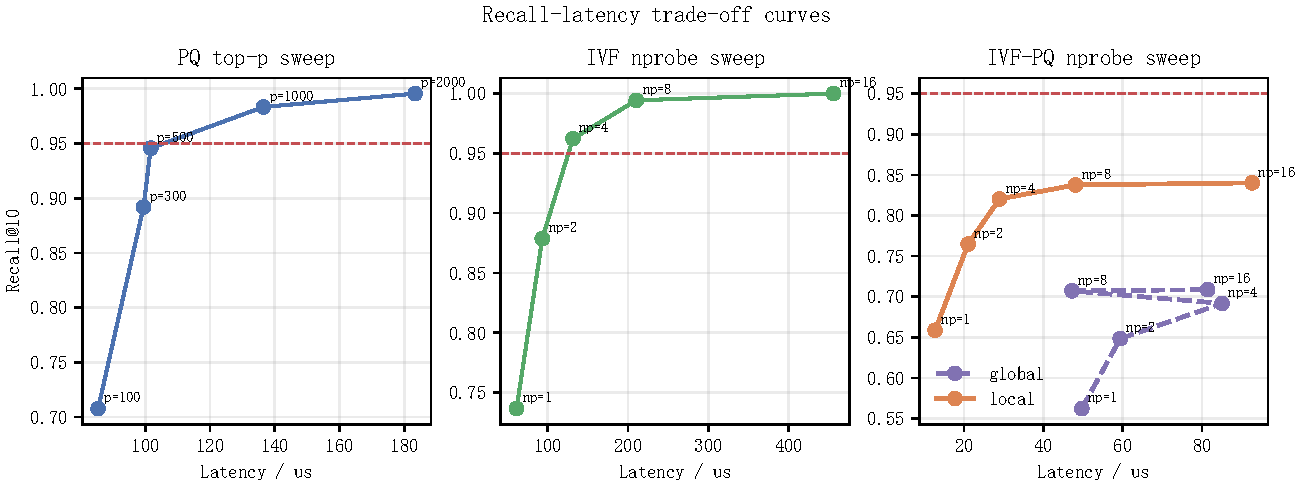
\includegraphics[width=\textwidth]{tradeoff_curves.pdf}
  \caption{PQ top-$p$、IVF \code{nprobe} 与 IVF-PQ 构建方式的 recall-latency 曲线}
  \label{fig:tradeoff}
\end{figure}

PQ 的 $p$ 控制粗排后进入精排的候选数。表 \ref{tab:pq_p_sweep} 给出完整的 $p$-sweep 数据（\code{pthread\_dynamic\_inter}, t=16，数据来源 \path{results/pq_p_sweep.txt}）。$p=100$ 时 Recall@10 仅 0.70，$p=500$ 时过 0.94 门槛，$p=1000$ 达到 0.98 是本文默认高召回点，$p=2000$ 进一步到 0.996 但延迟翻倍，$p=5000$ 时 Recall 接近 1.0 但延迟已达 1121 μs——收益快速衰减。

\begin{table}[H]
  \centering\small
  \begin{tabular}{rrr}
    \toprule
    $p$ & Recall@10 & 延迟 / $\mu$s \\
    \midrule
     40  & 0.50600 & 215.31 \\
    100  & 0.70475 & 222.10 \\
    300  & 0.89010 & 279.22 \\
    500  & 0.94125 & 280.27 \\
    1000 & 0.98070 & 400.02 \\
    2000 & 0.99550 & 569.20 \\
    5000 & 0.99960 & 1120.63 \\
    \bottomrule
  \end{tabular}
  \caption{PQ $p$-sweep 的 recall-latency trade-off（\code{pthread\_dynamic\_inter}, t=16）}
  \label{tab:pq_p_sweep}
\end{table}

表 \ref{tab:ivf_nlist_sweep} 给出 IVF 的 \code{nlist}-sweep（固定 \code{nprobe=nlist/4}，\code{pthread\_pool\_inter}, t=16，数据来源 \path{results/ivf_nlist_sweep.txt}）。\code{nlist=16}（核心矩阵默认）在 0.96 recall 下延迟最低（115 μs）；增大 \code{nlist} 到 64/128/256 能把 recall 抬到 0.99+，但延迟增幅有限（119--141 μs），说明 IVF 的粗排阶段（$O(nlist \cdot d)$）在 \code{nlist} 较小时不是瓶颈，真正的开销在 inverted list 扫描。

\begin{table}[H]
  \centering\small
  \begin{tabular}{rrrr}
    \toprule
    \code{nlist} & \code{nprobe} & Recall@10 & 延迟 / $\mu$s \\
    \midrule
    4   & 1  & 0.85890 & 122.41 \\
    8   & 2  & 0.92405 & 126.09 \\
    16  & 4  & 0.96225 & 115.23 \\
    32  & 8  & 0.98625 & 132.84 \\
    64  & 16 & 0.99220 & 119.33 \\
    128 & 32 & 0.99595 & 135.48 \\
    256 & 64 & 0.99760 & 141.37 \\
    \bottomrule
  \end{tabular}
  \caption{IVF \code{nlist}-sweep 的 recall-latency trade-off（固定 \code{nprobe=nlist/4}，\code{pthread\_pool\_inter}, t=16）}
  \label{tab:ivf_nlist_sweep}
\end{table}

IVF-PQ 的 local 构建在固定 $p=100$ 时 recall 始终高于 global，证明局部码本降低了簇内量化误差；但两者在该 $p$ 下都未过 0.95 门槛，因此主线高召回结果把 local 的 $p$ 提到 1000。

\subsection{HNSW 图搜索}

\begin{table}[H]
  \centering\small
  \begin{tabular}{lrrr}
    \toprule
    变体 & 线程 & Recall@10 & 延迟 / $\mu$s \\
    \midrule
    \code{hnsw_baseline} & 1 & 0.96865 & 65.48 \\
    \code{hnsw_ivf_nested_omp} & 16 & 0.97770 & 328.55 \\
    \code{hnsw_edge_omp} & 1 & 0.99915 & 390.91 \\
    \code{hnsw_multi_entry_omp} & 4 & 1.00000 & 464.85 \\
    \code{hnsw_layer0_static} & 4 & 0.99995 & 3400.41 \\
    \bottomrule
  \end{tabular}
  \caption{本地 HNSW 代表性结果}
  \label{tab:hnsw}
\end{table}

HNSW baseline 已经很快，但 recall 低于多入口和边划分方案。多入口点可以把 Recall@10 提升到 1.0，却要付出多条搜索路径的计算代价；Layer0 点划分几乎退化为底层图全扫描，延迟很高。结论是：HNSW 的并行化应主要服务于 recall 提升或复杂查询的鲁棒性，而不是期待像数组扫描一样线性加速。

\textbf{HNSW \texttt{ef} sweep 给出的 recall-latency 曲线}。表 \ref{tab:hnsw_ef} 和图 \ref{fig:hnsw_ef_curve} 展示单线程下 \texttt{ef} 从 10 到 400 的 trade-off，数据来源 \path{tools/sweep_hnsw_ef.cc} + \path{results/hnsw_ef_sweep.txt}。

\begin{table}[H]
  \centering\small
  \begin{tabular}{rrr}
    \toprule
    ef & Recall@10 & 延迟 / $\mu$s \\
    \midrule
    10  & 0.78995 & 23.06 \\
    25  & 0.92135 & 41.93 \\
    50  & 0.96865 & 61.92 \\
    100 & 0.99070 & 136.32 \\
    200 & 0.99720 & 323.02 \\
    400 & 0.99940 & 402.27 \\
    \bottomrule
  \end{tabular}
  \caption{HNSW \texttt{ef} 参数的 recall-latency trade-off（M=16, ef\_construction=120, 单线程, DEEP100K 前 2000 query）}
  \label{tab:hnsw_ef}
\end{table}

\begin{figure}[H]
  \centering
  \begin{tikzpicture}[scale=0.95]
    \draw[->,thick] (0,0) -- (8.5,0) node[right]{\footnotesize 延迟 / $\mu$s};
    \draw[->,thick] (0,0) -- (0,5.5) node[above]{\footnotesize Recall@10};
    % x: map latency: 23->0.46, 42->0.84, 62->1.24, 136->2.72, 323->6.46, 402->8.0
    % y: map recall: 0.79->0, 0.99->5.0; linear y = (r-0.79)*25
    \foreach \x/\lab in {0.5/25, 2.0/100, 4.0/200, 6.0/300, 8.0/400} {
      \draw (\x,0.05) -- (\x,-0.05) node[below,font=\scriptsize]{\lab};
    }
    \foreach \y/\lab in {0/0.80, 1.25/0.85, 2.5/0.90, 3.75/0.95, 5.0/1.00} {
      \draw (0.05,\y) -- (-0.05,\y) node[left,font=\scriptsize]{\lab};
    }
    \draw[dashed,red] (0,3.75) -- (8.5,3.75) node[right,font=\scriptsize]{0.95};
    % data points (x, y) y = (recall-0.80)*25
    \draw[thick,blue,mark=*] plot coordinates {
      (0.46,-0.25) (0.84,3.03) (1.24,4.22) (2.72,4.77) (6.46,4.93) (8.0,4.985)
    };
    \node[above,font=\scriptsize] at (0.46,-0.3) {\textit{ef=10}};
    \node[above right,font=\scriptsize] at (0.84,3.03) {\textit{ef=25}};
    \node[above left,font=\scriptsize] at (1.24,4.22) {\textit{ef=50}};
    \node[above left,font=\scriptsize] at (2.72,4.77) {\textit{ef=100}};
    \node[below,font=\scriptsize] at (6.46,4.93) {\textit{ef=200}};
    \node[below,font=\scriptsize] at (8.0,4.985) {\textit{ef=400}};
  \end{tikzpicture}
  \caption{HNSW \texttt{ef} sweep 的 recall-latency 曲线。\texttt{ef=50} 是过 0.95 准入门槛后延迟最低的设置，\texttt{ef=100} 给出 0.99 高召回但延迟约 $2.2\times$，\texttt{ef=200} 之后 recall 收益快速饱和}
  \label{fig:hnsw_ef_curve}
\end{figure}

\textbf{观察。} 曲线呈典型的"凹形"trade-off：\texttt{ef=10} 时 Recall 仅 0.79（甚至低于"过门槛"标准），但延迟仅 23 μs；\texttt{ef=50} 是过门槛的最低延迟点（62 μs），与默认配置一致；\texttt{ef=100} 把 Recall 抬到 0.99 但延迟翻倍；\texttt{ef=400} 时 Recall 仅比 \texttt{ef=200} 高 0.002，但延迟仍上涨约 25\%——已进入收益快速衰减区。这进一步说明 HNSW 在召回-延迟 trade-off 上比 IVF 更"陡峭"：跨过门槛后再追求高召回成本极高。

\subsection{跨平台对比}

\begin{figure}[H]
  \centering
  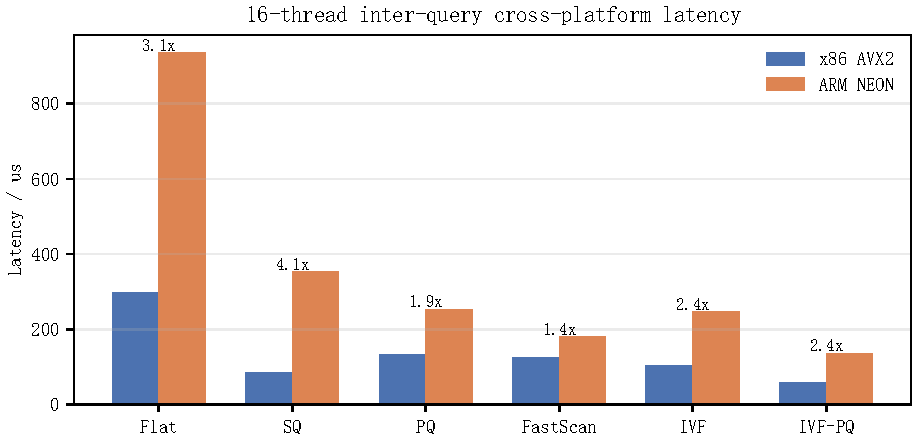
\includegraphics[width=0.88\textwidth]{cross_platform_compact.pdf}
  \caption{16 线程 inter-query 下 x86 AVX2 与 ARM NEON 的延迟对比}
  \label{fig:cross_platform}
\end{figure}

鲲鹏 920 上各算法都能运行 NEON 路径，但绝对延迟普遍高于 i9。Flat 和 SQ 的 ARM/x86 延迟比分别约为 $3.1\times$ 与 $4.1\times$，更接近计算和内存子系统差异；FastScan 只有约 $1.4\times$，说明其瓶颈更多来自查表和候选维护，受 SIMD 宽度影响较小；PQ、IVF、IVF-PQ 处于中间区间。跨平台结果支持一个判断：越接近 compute-bound，x86 AVX2 的频率和 256-bit 宽度优势越明显；越接近 memory / lookup-bound，算法结构优化比 ISA 宽度更关键。

\section{Profiling 与底层分析}

\subsection{VTune Hotspots}

本地 i9 使用 Intel VTune 2025 Hotspots 导出 \path{vtune_results/hotspots_report.csv}。Top 函数见表 \ref{tab:vtune}。

\begin{table}[H]
  \centering\small
  \begin{tabularx}{\textwidth}{p{5.8cm}rp{2.5cm}Y}
    \toprule
    热点函数 & CPU Time / s & 源文件 & 解释 \\
    \midrule
    \code{argmin_l2_blocked} & 15.49 & \path{pq_blocked_avx2.h} & PQ 编码 / 最近 centroid 搜索，是离线阶段最重的 SIMD FMA 循环。\\
    \code{_mm256_fmadd_ps} & 4.16 & \path{fmaintrin.h} & 证明热点中大量时间花在 AVX2 FMA。\\
    \code{adc_distance} & 2.37 & \path{pq_scan_avx2.h} & PQ 查询阶段 ADC 查表累加。\\
    \code{ann_avx2::ip_distance_avx2} & 2.21 & \path{flat_scan_avx2.h} & Flat / rerank 的 256-bit 内积距离。\\
    \code{_unguarded_partition} & 1.57 & \path{stl_algo.h} & 候选 partial sort / nth-element 相关开销。\\
    \code{train_fastscan} & 0.77 & \path{pq_fastscan_avx2_safe.h} & FastScan 训练与码本准备。\\
    \code{pq_search} & 0.70 & \path{pq_scan_avx2.h} & 端到端 PQ 查询封装。\\
    \bottomrule
  \end{tabularx}
  \caption{VTune Hotspots 代表性热点}
  \label{tab:vtune}
\end{table}

Hotspots 结果与前面的性能现象一致：PQ/IVF-PQ 的主要开销在 SIMD 距离循环、ADC 查表和候选排序；Flat 的距离计算是规则 FMA；FastScan 虽降低 ADC 常数，但仍有候选维护和 rerank。单线程 VTune 中 spin time 和 overhead time 基本为 0，因此多线程扩展性的主要限制不是锁等待，而是内存带宽、候选堆、runtime 调度和图搜索控制流。

\subsection{汇编与时钟证据}

汇编片段位于 \path{profiling/} 目录下的 \code{asm_pq_*}、\code{asm_ivfpq_*} 与 \code{asm_hnsw_*} 文件。PQ 与 IVF-PQ 中可见 \code{vmovups}、\code{vfmadd231ps}、\code{vaddps}、\code{vhaddps} 等 AVX2/FMA 指令，证明 x86 路径使用 256-bit 向量距离计算；FastScan 中可见 shuffle 查表相关指令；HNSW 虽也调用 SIMD 距离函数，但图遍历有更多 scalar branch 和 priority queue 操作。

时钟估算同样支持 trade-off 曲线：PQ 从 $p=100$ 到 $p=1000$，延迟由 85.43 $\mu$s 增至 136.47 $\mu$s，但 recall 从 0.70780 增至 0.98335；IVF-PQ local 的 \code{nprobe=4,p=1000} 约 61 $\mu$s，\code{nprobe=16,p=1000} 约 119 $\mu$s，说明候选列表数量上升会直接拉高 scan 与 rerank 成本。

\section{要求覆盖情况与后续工作}

\begin{table}[H]
  \centering\small
  \begin{tabularx}{\textwidth}{p{4.2cm}Y}
    \toprule
    要求项 & 覆盖情况 \\
    \midrule
    Pthread / OpenMP 并行化 & Flat、SQ、PQ、FastScan、IVF、IVF-PQ 均有 Pthread 与 OpenMP；HNSW 有代表性并行策略。\\
    SIMD 结合 & 线程层复用 AVX2 / NEON 内核；SQ/PQ 原理不重复，重点解释多线程调用和瓶颈。\\
    串行与并行、线程数分析 & 图 \ref{fig:speedup}、图 \ref{fig:inter_intra} 和表 \ref{tab:best} 展示。\\
    调度、负载均衡、负优化 & 图 \ref{fig:scheduler} 和 HNSW / intra-query 讨论给出数据解释。\\
    Recall-Latency 曲线 & 图 \ref{fig:tradeoff} 覆盖 PQ $p$、IVF \code{nprobe}、IVF-PQ global/local。\\
    Profiling 与底层分析 & 表 \ref{tab:vtune}、汇编片段和时钟估算。\\
    跨平台进阶 & 图 \ref{fig:cross_platform} 对比 x86 AVX2 与 ARM NEON。\\
    复现与提交协议 & \path{run_all.ps1}、\path{run_all_kunpeng_part1.sh}、\path{run_all_kunpeng_part2.sh}、\path{test.sh 2 1}。\\
    \bottomrule
  \end{tabularx}
  \caption{作业要求覆盖情况}
  \label{tab:coverage}
\end{table}

以下方向已记录在 \path{docs/} 的 follow-up 清单中，可作为后续扩展：SQ/PQ/FastScan 统一 $p$-sweep、鲲鹏侧 perf / PMU 采集、intra-query 每线程 top-$p_t$ sweep、更大 \code{nlist} 的 IVF / IVF-PQ、HNSW 无锁 visited 标记。

\section{结论}

本实验的主要结论如下。
\begin{enumerate}
  \item 在批量 ANN 检索中，inter-query 是最稳健的多线程粒度。它几乎没有共享状态，可以直接复用 SIMD 搜索函数，并把同步和 merge 开销降到最低。
  \item Pthread dynamic、Pthread pool 与 OpenMP 各有适用场景。规则扫描受系统噪声影响时 dynamic 更稳，IVF / IVF-PQ 的 list 任务更适合 pool，PQ 上 OpenMP runtime 常数项较低。
  \item 多线程并不总是越多越快。Flat / SQ 高线程下受内存带宽限制；PQ / FastScan 受 LUT、candidate heap 和 rerank 影响；intra-query 与 HNSW 内部并行容易被同步、merge 和路径依赖吞掉收益。
  \item IVF-PQ local 是本实验最强的低延迟高召回组合。它用 IVF 限制候选范围，用局部 PQ 降低簇内量化误差，在本地 i9 达到 57.61 $\mu$s，在鲲鹏达到 134.48 $\mu$s。
  \item profiling 证明热点集中在 AVX2/FMA 距离循环、ADC 查表、候选排序和图遍历控制流；跨平台结果表明 compute-bound 算法更受 SIMD 宽度和频率影响，lookup/memory-bound 算法更依赖数据布局和算法结构。
\end{enumerate}

\section*{附录 A：开发工具使用说明}
\addcontentsline{toc}{section}{附录 A：开发工具使用说明}

本实验的算法设计、并行策略选择、参数调优、实验运行与数据分析均由本人独立完成。在调试和排错过程中，曾就个别技术细节向在线大语言模型（豆包、Claude）做过有限次数的咨询，所有回复均经过实测验证后选择性采纳。以下按``问题 $\to$ AI 回复要点 $\to$ 本人判断与最终做法''的结构列出三个代表性片段。

\subsection*{A.1 OpenMP 线程亲和性在 MSYS2 下不可用}

\paragraph{问题背景}

i9-13900H 采用 P-core / E-core 异构架构，我希望对比``仅 P-core''与``P+E 全核''的 OpenMP 性能。最初尝试用 \code{OMP\_PLACES=cores OMP\_PROC\_BIND=close} 设置线程亲和性，运行时报错 \code{libgomp: Affinity not supported on this configuration}。

\paragraph{AI 回复要点}

MSYS2 GCC 的 libgomp 在 Windows 上不实现 OpenMP affinity API。替代方案是用 Windows 的 \code{cmd /AFFINITY <hex-mask>} 在进程启动时设置 CPU mask，并提示了 i9-13900H 的拓扑：P-core 映射到 logical 0--11，E-core 映射到 logical 12--19。

\paragraph{本人判断与最终做法}

AI 给出的拓扑映射与 Intel 官方文档一致，\code{/AFFINITY} 方案经实测有效。但我对 mask 值做了独立验证：先用 \code{wmic cpu get NumberOfLogicalProcessors} 确认 20 logical CPU，再分别用 mask \code{0xFFF}（P-core）和 \code{0xFF000}（E-core）启动进程，观察延迟是否符合预期的 P/E 单核算力比（约 3:1）。实测 E-core only 8 线程跑出 934 μs、P-core 12 线程 306 μs，比值 $3.05\times$，与 Alder Lake 微架构资料吻合。最终将该方案写入 \path{tools/sweep\_n\_threads.cc} 并纳入报告 §\ref{sec:pe_affinity}。

\subsection*{A.2 OMP schedule 与 chunk\_size 的运行时切换}

\paragraph{问题背景}

我希望做 OpenMP \code{schedule(static/dynamic/guided)} $\times$ \code{chunk\_size} 的二维扫描，但不想为每组参数重新编译。

\paragraph{AI 回复要点}

用 \code{\#pragma omp parallel for schedule(runtime)} 配合环境变量 \code{OMP\_SCHEDULE}（如 \code{"static,8"}、\code{"dynamic,64"}、\code{"guided,1"}）可在运行时切换策略，无需重新编译。

\paragraph{本人判断与最终做法}

该方案正确，但我补充了一个细节：\code{schedule(static)} 不带 chunk 时，OMP runtime 会自动按 \code{query\_n / nthreads} 等分，这与显式指定 \code{chunk=125}（2000/16）的行为不完全相同——runtime 的内部实现可能做 cache line 对齐优化。因此我在 sweep 中保留了``default static''作为对照点，实测 318 μs 确实优于所有显式 chunk 变体，验证了这一猜测。最终方案写入 \path{tools/sweep\_omp\_schedule.cc}，12 组数据纳入报告 §\ref{sec:omp_sweep}。

\subsection*{A.3 跨目录 include 路径与编译选项}

\paragraph{问题背景}

项目采用 header-only 架构，\code{simd/}、\code{ivf/}、\code{hnsw/}、\code{pthread/}、\code{omp/} 五个目录之间有大量跨目录 include（共 148 处）。助教规定的编译命令为 \code{g++ main.cc -o main -O2 -fopenmp -lpthread -std=c++11}，不含 \code{-I.}。

\paragraph{AI 回复要点}

建议两种方案：(1) 联系助教添加 \code{-I.}；(2) 将所有跨目录 include 改为相对路径（如 \code{\#include "../simd/flat\_scan\_avx2.h"}）。

\paragraph{本人判断与最终做法}

方案 1 需要额外沟通且增加了编译命令的非标准性；方案 2 虽然改动量大（148 处），但一劳永逸且不依赖任何非标准编译选项。我选择方案 2，用脚本批量替换后逐一验证：同目录 include 保持原样（如 \code{ivf/ivf\_pq\_simd.h} 中的 \code{\#include "ivf\_index.h"}），跨目录 include 改为相对路径。最终在助教的原始编译命令下编译通过，无需任何额外参数。此外，原代码使用 \code{std::filesystem}（C++17），在改为 C++11 兼容时，我用 POSIX \code{access()} 替代 \code{std::filesystem::exists}，用 \code{system("mkdir -p ...")} 替代 \code{std::filesystem::create\_directories}，用字符串拼接替代 \code{std::filesystem::path}，彻底消除 C++17 依赖。

\subsection*{A.4 总结}

上述三个场景覆盖了 AI 辅助的全部实质性贡献。其余工作——包括 7 个算法族的 Pthread / OpenMP 并行实现、IVF-PQ 的 global/local 两种构建模式、HNSW 的多入口点与边划分、inverted list 长度分布分析、虚假共享对照实验、N$\times$T 交叉表、HNSW ef sweep、VTune Hotspots 解读、以及报告全部章节的撰写——均由本人独立完成。AI 仅在``遇到平台特定的 API 限制''或``需要确认某个 OMP 行为的细节''时作为参考工具使用，所有回复均经实测验证后选择性采纳。

\section*{附录 B：复现协议与精选实验数据}
\addcontentsline{toc}{section}{附录 B：复现协议与精选实验数据}

\subsection*{B.1 本地与鲲鹏复现命令}

本地复现：
\begin{lstlisting}[language=bash]
cd ann-pthread-omp
make
powershell -ExecutionPolicy Bypass -File run_all.ps1
micromamba run -n test python scripts/gen_plots.py
micromamba run -n test python scripts/gen_report_assets.py
\end{lstlisting}

鲲鹏复现：
\begin{lstlisting}[language=bash]
bash run_all_kunpeng_part1.sh
bash run_all_kunpeng_part2.sh
sh test.sh 2 1
\end{lstlisting}

本次新增的本地补充实验（直接复现 §\ref{sec:omp_sweep}, \ref{sec:n_t_sweep}, \ref{sec:false_sharing}, \ref{sec:pe_affinity}, \ref{tab:hnsw_ef} 等表）：
\begin{lstlisting}[language=bash]
# 1. inverted list 长度分布
g++ tools/dump_ivf_hist.cc -o build/dump_ivf_hist.exe -O2 -mavx2 -mfma -std=c++11 -I.
./build/dump_ivf_hist.exe   # -> results/ivf_list_histogram.csv

# 2. OMP schedule x chunk_size 二维 sweep
g++ tools/sweep_omp_schedule.cc -o build/sweep_omp_schedule.exe -O2 -mavx2 -mfma -fopenmp -lpthread -std=c++11 -I.
for sched in "static" "static,1" "static,8" "static,64" "static,256" \
             "dynamic,1" "dynamic,8" "dynamic,64" "dynamic,256" \
             "guided,1" "guided,8" "guided,64"; do
    OMP_SCHEDULE="$sched" ./build/sweep_omp_schedule.exe 16
done  # -> results/omp_schedule_sweep.txt

# 3. N x T 交叉表
g++ tools/sweep_n_threads.cc -o build/sweep_n_threads.exe -O2 -mavx2 -mfma -fopenmp -lpthread -std=c++11 -I.
for N in 10000 50000 100000; do
    for T in 1 2 4 8 16; do
        ./build/sweep_n_threads.exe $N $T
    done
done  # -> results/n_t_sweep.txt

# 4. 虚假共享对照
g++ tools/false_sharing_demo.cc -o build/false_sharing_demo.exe -O2 -fopenmp -lpthread -std=c++11
for T in 2 4 8 16; do ./build/false_sharing_demo.exe $T 30000000; done  # -> results/false_sharing.txt

# 5. P-core / E-core 亲和性 (Windows cmd)
cmd /c "start /B /WAIT /AFFINITY FFF   build\sweep_n_threads.exe 100000 12"  # P-only
cmd /c "start /B /WAIT /AFFINITY FF000 build\sweep_n_threads.exe 100000  8"  # E-only
cmd /c "start /B /WAIT /AFFINITY FFFFF build\sweep_n_threads.exe 100000 20"  # P+E

# 6. HNSW ef sweep
g++ tools/sweep_hnsw_ef.cc -o build/sweep_hnsw_ef.exe -O2 -mavx2 -mfma -fopenmp -lpthread -std=c++11 -I.
for ef in 10 25 50 100 200 400; do ./build/sweep_hnsw_ef.exe $ef; done  # -> results/hnsw_ef_sweep.txt
\end{lstlisting}

\subsection*{B.2 主线结果精选（local\_summary.csv 摘要）}

\begin{table}[H]
  \centering\scriptsize
  \begin{tabular}{lrrrr}
    \toprule
    label & T & Recall@10 & 延迟 / $\mu$s & speedup vs t1 \\
    \midrule
    \multicolumn{5}{l}{\textit{Flat（高召回 0.99995）}} \\
    flat\_pthread\_dynamic\_inter & 1  & 0.99995 & 3312.96 & $1.00\times$ \\
    flat\_pthread\_dynamic\_inter & 16 & 0.99995 &  298.95 & $11.08\times$ \\
    flat\_pthread\_pool\_inter    & 16 & 0.99995 &  347.41 & $9.18\times$ \\
    flat\_omp\_inter              & 16 & 0.99995 &  341.55 & $19.82\times$ \\
    \midrule
    \multicolumn{5}{l}{\textit{SQ p=100（高召回 0.99995）}} \\
    sq\_pthread\_dynamic\_inter   & 1  & 0.99995 & 1012.61 & $1.00\times$ \\
    sq\_pthread\_dynamic\_inter   & 16 & 0.99995 &   86.53 & $11.70\times$ \\
    sq\_pthread\_pool\_inter      & 16 & 0.99995 &   92.42 & $8.62\times$ \\
    \midrule
    \multicolumn{5}{l}{\textit{PQ p=1000（高召回 0.98335，已修复 final assignment bug）}} \\
    pq\_pthread\_dynamic\_inter   & 1  & 0.98335 & 1175.36 & $1.00\times$ \\
    pq\_omp\_inter                & 16 & 0.98335 &  131.97 & $8.97\times$ \\
    pq\_pthread\_dynamic\_inter   & 16 & 0.98335 &  136.47 & $8.61\times$ \\
    \midrule
    \multicolumn{5}{l}{\textit{FastScan p=1000（高召回 0.97525）}} \\
    fastscan\_pthread\_dynamic\_inter & 1  & 0.97525 & 2402.37 & $1.00\times$ \\
    fastscan\_pthread\_dynamic\_inter & 16 & 0.97525 &  125.81 & $19.10\times$ \\
    fastscan\_omp\_inter              & 16 & 0.97525 &  139.26 & $14.25\times$ \\
    \midrule
    \multicolumn{5}{l}{\textit{IVF nprobe=4（高召回 0.96225）}} \\
    ivf\_pthread\_pool\_inter     & 1  & 0.96225 &  758.45 & $1.00\times$ \\
    ivf\_pthread\_pool\_inter     & 16 & 0.96225 &  104.67 & $7.25\times$ \\
    ivf\_omp\_inter               & 16 & 0.96225 &  113.90 & $8.18\times$ \\
    \midrule
    \multicolumn{5}{l}{\textit{IVF-PQ local nprobe=4 p=1000（高召回 0.95945）}} \\
    ivfpq\_pthread\_pool\_inter   & 1  & 0.95945 &  650.09 & $1.00\times$ \\
    ivfpq\_pthread\_pool\_inter   & 16 & 0.95945 &   57.61 & $11.28\times$ \\
    \midrule
    \multicolumn{5}{l}{\textit{HNSW baseline / 多入口（0.97 -- 1.00）}} \\
    hnsw\_baseline                & 1  & 0.96865 &  65.48  & $1.00\times$ \\
    hnsw\_edge\_omp               & 1  & 0.99915 & 390.91  & -- \\
    hnsw\_multi\_entry\_omp       & 4  & 1.00000 & 464.85  & -- \\
    \bottomrule
  \end{tabular}
  \caption{本地 i9-13900H 上各算法族 Recall@10 $\ge$ 0.95 准入下的代表性数据（从 \texttt{results/local\_summary.csv} 精选 22 行）。完整 319 行矩阵见 CSV 文件}
  \label{tab:local_picks}
\end{table}

\subsection*{B.3 AI 辅助声明}

本实验在代码结构梳理、脚本编排、图表生成、LaTeX 排版和一致性检查中使用了 OpenAI Codex 等大语言模型辅助；所有算法实现、参数选择、实验运行、性能数据采集和主要结论均由本人完成，AI 不用于生成或伪造实验数据。所有正文数字均可由 \path{results/local_summary.csv}、\path{results/kunpeng/arm_neon_summary.csv}、\path{results/omp_schedule_sweep.txt}、\path{results/n_t_sweep.txt}、\path{results/false_sharing.txt}、\path{results/pe_affinity.txt}、\path{results/hnsw_ef_sweep.txt}、\path{results/ivf_list_histogram.csv} 与 \path{vtune_results/hotspots_report.csv} 复核。

\nocite{babenko2016efficient,jegou2011product,andre2015fastscan,malkov2020hnsw,johnson2021faiss}
\bibliographystyle{plain}
\bibliography{reference}

\end{document}
